\documentclass[a4paper]{article}

\usepackage[T1]{fontenc}
\usepackage[english]{babel}
\usepackage{textcomp}
\usepackage{multirow}
\usepackage{float}
\usepackage{fancyhdr}
\usepackage{pdfpages}
\usepackage{graphicx}
\usepackage{amsmath}

\title{DH2320 Lab work}
\author{Karl Johan Andreasson <{kalleand@kth.se}> %
\and Mikaela N\"oteberg <{mnot@kth.se}>
}

\fancyhf{}
\fancyhead[LE,RO]{\slshape \rightmark}
\fancyhead[LO,RE]{\slshape \leftmark}
\fancyfoot[C]{\thepage}

\begin{document}
\thispagestyle{empty}
\maketitle
\thispagestyle{empty}
\pagestyle{empty}
\newpage
\pagestyle{fancy}
\setcounter{page}{1}

\section{Lab 1: WebGL and Three.js}
\subsection{Make the first cube look like the second one.}

For the first assignment we were supposed to alter how a Javascript using WebGL rendered a
cube to look more like what it did using the Javascript library Three.js.

To do this we changed the position of the cube further away from the perspective
camera located in the origin of the coordinate system. We changed the Z-value
from $-2$ to $-8$, this made the whole cube visible.

This was not enough as we needed a rotation around the y-axis as well as
rotation around the x-axis. To do this we added the snippet:

\begin{verbatim}
mat4.rotate(mvMatrix, rCube/2, [ 0, 1, 0 ]);
\end{verbatim}

\subsection{Adding a tetrahedron}

In the next assignment we added a tetrahedron to both scenes. To accomplish this
we moved the cubes in both scenes to the left by $1.5$ units. Then we added the
Three.js tetrahedron by adding a TetrahedronGeometry with the size of 1.5 units.

The tetrahedron implemented using the vertices:

\begin{verbatim}
(1, 1, -1)
(1, -1, 1)
(-1, 1, 1)
(-1, -1, -1)
\end{verbatim}

The radius of the circumsphere for this tetrahedron is $\approx 1.73$ which is
the value we used when initiating the tetrahedron in the Three.js version.

In the WebGL version this was a lot trickier as we had to figure out where the
vertices where located in a tetrahedron with a certain size.

The rotation around x-axis was set to be the same for the tetrahedron as the
cube. The rotation around z-axis was set to be negative speed of the rotation
around x-axis divided by 2. The tetrahedron, in contrast to the cube, was set to
not rotate around the y-axis.

The colors were fixed to match in both scenes through trial and error mostly.
\newpage
\section{Lab 2: Photoshop Techniques}
Using mostly Photoshop and some GIMP we restored and altered a number of pictures.

\subsection{Image restoration} % baby, scratched, pink flowers, marsvin
The image restoration involved a faded baby, a scratched photo of a mother and a
baby, a photo of pink flowers, and a photo of a guinea pig. For the baby we
added an adjustment layer to correct the faded colors. We also did some
sharpening, altering the contrasts, and added a circular gradient with high
opacity to even out the edges of the photo.

To restore the scratched photo it was sufficient to use the \textbf{clone
stamp}. We removed the damage on the right hand side and removed all of the
highly visible dirt and scratches. The pink flowers changed color to blue using
the \textbf{replace color} adjustment tool. The guinea pig photo was done in a
similar way as the first photo. We altered the color balance to our liking and
by that made sure the kid is interpreted as the subject of the image. While
altering the colors we made sure that the photo was not perceived as flat as in
the original photo. This made the subject of the photo much clearer, being in
center and all.

\subsection{Retouching} % phat
Using the \textbf{elliptical marquee} in conjunction with the \textbf{liquify}
filter to narrow the figure of the model in \textit{Phat.png}. We mostly work on
his stomach, but made som over-all narrowing of his figure, neck and chin. At
some places the distortion became too large, but this was easily fixed with the
\textbf{reconstruction tool}.

\subsection{Creating a seamless tile} % wood
Working on \textit{Wood.png} involved both Photoshop and GIMP. In Photoshop we
cropped the image to a suitable square form, resized it and did some retouching
to i.e. remove the coffee stain. After reading the \textit{Seamless tile
tutorials} from the course web page we found that GIMP had the most convenient
approach to making something seamless, and therefore we exported the pre-worked
tile there and used the \textbf{Filters>Map>Make Seamless} command to finish our
seamless tile.

\subsection{Montage and design} % poster
We made a poster for a post-apocalyptic event (inspired by Fallout and
Borderlands). We started out with three images of a destroyed city, pip-boy and
uncle Sam respectively. Working with texts, layers and filters we aimed for the
design of an old and somewhat worn poster. The pip-boy image to the far right is
intended to be interpreted as a sticker applied to the poster.

\subsection{Webpage} % adding structure to cube in three.js
Using the seamless wooden tile constructed earlier we added texture to the
rotating cube in a copy of the Three.js parts of our first lab. To apply the
texture to the cube we changed the materials to mapping a texture. Since we
wanted the same texture on all six surfaces of the cube, we no longer needed six
different materials. We then added repeating of the texture and set the repeat
to two times in both axes. See source code for implementation details.

\section{Lab 3: 3D Modelling and animation}

\subsection{A ball bouncing on a table} % Maya
Using Maya we modeled a ball bouncing on a table. The most advanced shape
involved was the table  which consists of several altered \textbf{cube
primitives}. The table top is a simple rectangular cube primitive with its top
face extruded (after texturing) and slightly altered to create a beveled shape.
The legs are copies of one modeled shape, which also was a cube primitive but
with more than one (five to be exact) division along its height. Using these
divisions, some simple scaling of the existing levels of four vertices each
created a sort of angled lathed table leg. Using \textbf{planar mapping} on
surfaces and \textbf{Phong} materials, we could texture the table with our
seamless tile from the second lab. On the legs we used \textbf{cylindrical
mapping}.

The ball itself is a straight on \textbf{sphere primitive} colored pink with
\textbf{Phong} material. In contrast to the table's \textit{face} normals the
ball has \textit{average} normals so that it will not be flat shaded. 

\subsubsection{Animation}
After modelling the shapes, the next step was to animate the ball bouncing on
the table. Using 60 frames the ball was to appear above the table, bounce on it
twice and then drop off. The bounces was set to be att approximately frame 20
and 40, i.e., a third and two thirds into the animation, and accordingly the
``extremes'' at frame 30 and 50. In the \textbf{Graph Editor} we made sure the
motion curve for the x-positions became a straight line. This way the speed of
the ball will be constant. To make the movement more like bouncing, we forced
the ball to change its y-direction immediately after hitting the table in each
bounce (still using the \textbf{Graph Editor}). This was done by splitting the
tangents at these points and alter the left-hand and right-hand side separately
to form a v-shape. 

\subsubsection{Lighting and rendering}
Lighting the scene was done by the basic principle of \textit{three-point
lighting}; a \textit{key light} to light the object (i.e., the ball), a
\textit{fill light} to light the rest of the scene, and a \textit{back light} to
distinguish foreground objects from background objects. We placed the
\textit{key light} in the upper-left front, the \textit{fill light} in the
upper-right front, and the \textit{back light} in the upper-left back, all
facing the middle of the table. To separate the different lights they have
different \textbf{intensities}. The \textit{back light} only has an intensity of
0.3 and the \textit{fill light} 0.5, while the \textit{key light} har full 1.0
intensity. Adding shadows was done by checking the \textbf{Use Depth Map
Shadows} box for all the light sources. Lastly the scene was rendered into a
movie file for viewing on the web page.

\subsection{Adding lights} % to webpage
\newpage
\section{Lab 4: Introduction to Data Mining}
The answers to the questions are available in the attached questionnaire. The
tables was charts were constructed following the lab assignment. Additional
charts or columns were created to answer certain questions in the questionnaire.
Below is how we reasoned about the questions.

Marking the S and M party one at a time in the straight table \textbf{Party} and
sorting the \textbf{Party Votes} on the column \textbf{Perc 2006} we could
answer the first four questions of the questionnaire, by selecting the top and
bottom Municipality.

Strongest municipality support overall in 2006 was selected from the bar chart
\textbf{Party votes}, with selections cleared.

Iterating over all the parties we noted the highest overall municipality support
was in Kalix (59.9\% for S).

Question 7, to achieve this we sorted on the column \textbf{Change} in
\textbf{Party Votes} with the party S investigated, marking the positive values
and noted the number in the text object.  Question 8 was achieved in a similar
manner as question 7, only to find no decreased support for M.

Question 9, we sorted on column \textbf{Participation} in \textbf{Vote overview
2006} and selected the highest value. Selecting that municipality (Lomma) the
answer to question 10 could be found in the bar chart \textbf{Party votes}.

Question 11 and 12, we simply sorted on column \textbf{Registered voters} in
\textbf{Vote overview 2006} and selected the top and bottom values.

To answer question 13 we added a new column \textbf{Perc blank} in \textbf{Vote
overview 2006} with the definition \textit{Sum(BlankVotes) / Sum(Voters)}. We
then sorted on this column and noted the highest percentage. Selecting that
municipality (Karlsborg) the answer to question 14 could be found in the bar
chart \textbf{Party votes}.

For question 15, a new straight table \textbf{Provinces} was created including
provinces. With the S party selected we sorted on column \textbf{Perc 2006} to
find the highest support. Sorting on column \textbf{Perc 2002} we found another
province at the top, which answered the next question.

We answered the next two questions in the same manner, but with the M party
selected instead.

To answer question 19 see selected \"Ovr and sorted on the highest percentage
both 2002 and 2006 and compared the top provinces. For the southern provinces we
mainly included Sk\aa ne, Blekinge and Halland. They were in the absolute top in
2006, but in 2002 it wasn't as clear.

Question 20, we played around with the municipalities where the support was
highest for each party and noted the participation percentage. The differences
were not high enough to make a definite statement about the trends noted.

\section{Lab 5: Introduction to 3D visualization}

\subsection{Visualizing a three-dimensional vector field}

\subsection{Analyzing the air quality of a kitchen}

\begin{enumerate}
    \item
        \begin{figure}
            \label{fig:dust}
            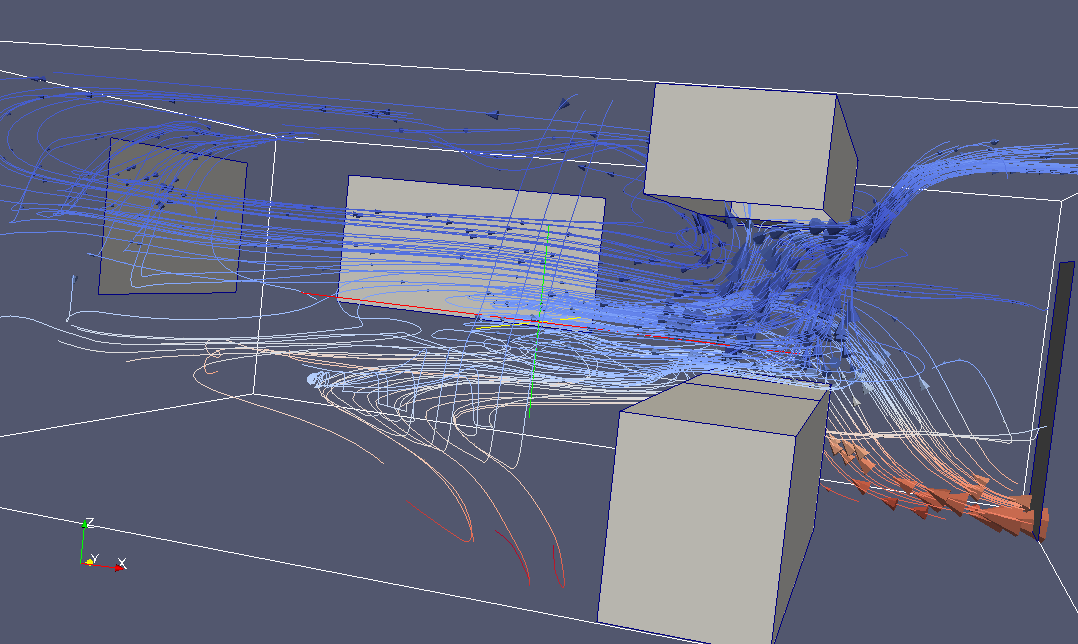
\includegraphics[width=1\linewidth]{lab5/kitchen-dust-screenshot.png}
            \caption{Dust gathering in the kitchen.}
        \end{figure}
        The most likely place the dust will settle are in the air filter in the
        kitchen fan and on the floor where the air velocity are low. In the
        figure \ref{fig:dust} we have visualized the air velocity and from it we can see
        that the air mainly comes from the door and escapes through the kitchen
        fan with some coming from the windows as well. The filter in the kitchen
        fan will therefore collect some of the dust. From the same image we can
        see that there are little to no air movement in the lower parts of the
        kitchen and particularly in the lower left and lower right part of the
        image the dust will probably collect.
    \item
        \begin{figure}
            \label{fig:pressure}
            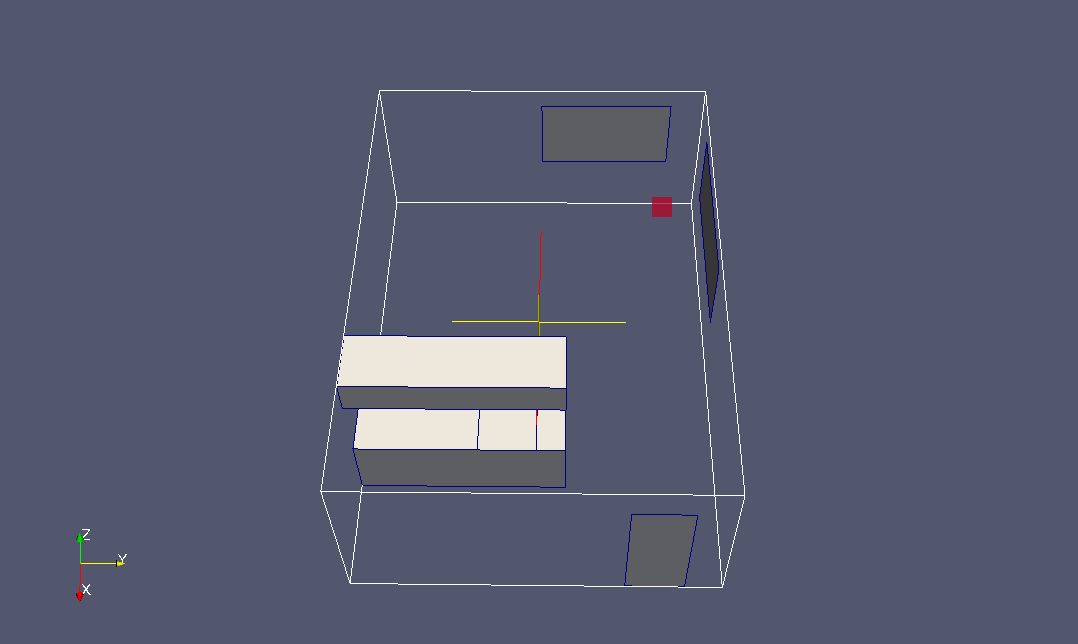
\includegraphics[width=1\linewidth]{lab5/kitchen-highest-pressure-screenshot.png}
            \caption{Highest air pressure.}
        \end{figure}
        The highest air pressure can be found in the figure \ref{fig:pressure}. The red dot
        in the image indicate where the air pressure is the highest. Generally
        the air pressure increases the closer to the ground we get. The highest
        air pressure value is 0.186993.
    \item
        \begin{figure}
            \label{fig:velocity}
            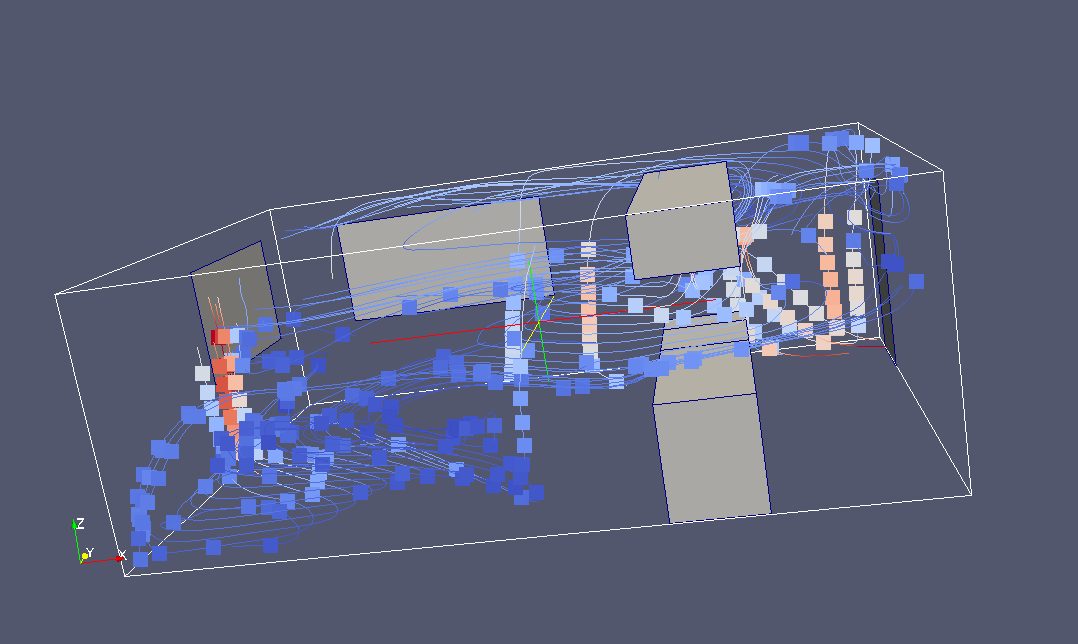
\includegraphics[width=1\linewidth]{lab5/kitchen-largest-air-velocity-screenshot.png}
            \caption{Highest air velocity.}
        \end{figure}
        As we can see in the figure \ref{fig:velocity} the highest air velocity are at the
        door, at the window in the opposite side of the door and at the kitchen
        fan. The absolutely highest air velocity can be found at the window and
        its numerical value is 0.067129.
\end{enumerate}

\subsection{Volume rendering}
\begin{figure}
    \label{fig:volume}
    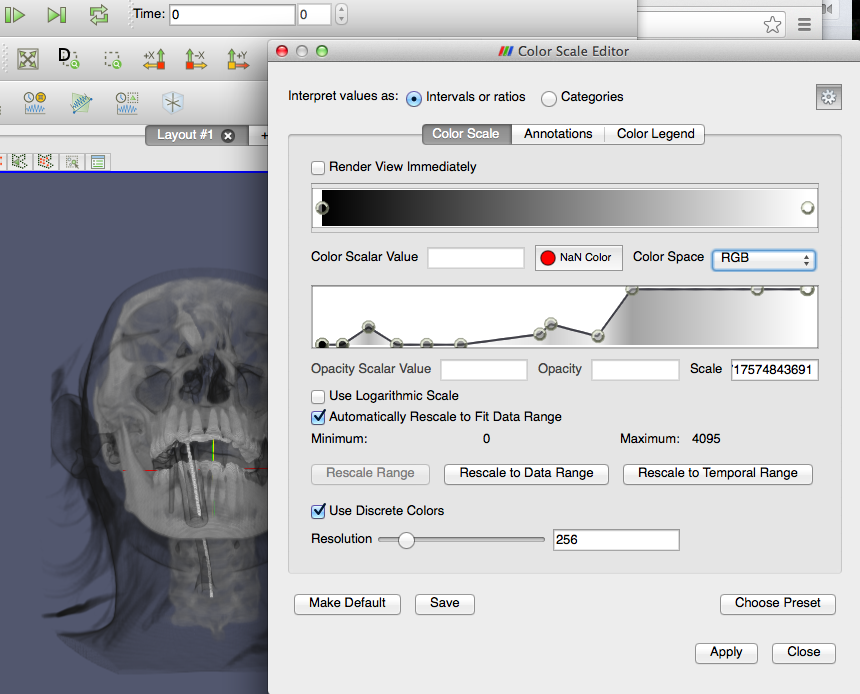
\includegraphics[width=1\linewidth]{lab5/head-transfer-function.png}
    \caption{Final transfer function.}
\end{figure}
We followed the lab assignments and reflected on what we did to use this to get
the end result shown in figure \ref{fig:volume}. The end result was achieved through
experimenting with the transfer function. We made the higher ranges of values
have quite high opacity and the lower ranges have lower. This made the skeleton
of the skull show with an indication of where the skin is located. The teeth
were shown by making the absolutely highest range of values have high opacity.

\end{document}
